%%%%%%%%%%%%%%%%%%%%%%%%%%%%%%%%%%%%%%%%%%%%%%%%%
% Chapter: Use Cases
%%%%%%%%%%%%%%%%%%%%%%%%%%%%%%%%%%%%%%%%%%%%%%%%%
\chapter{Use-Cases}
\label{app:use-cases}

The \ac{PMIx} standard provides many generic interfaces that can be composed into higher-level use cases in a variety of ways.  While the specific interfaces and attributes are standardized, the use cases themselves are not (and should not) be standardized.  Common use cases are included here as examples of how PMIx's generic interfaces \texttt{might} be composed together for a higher-level purpose. The use cases are intended for both \ac{PMIx} interface users and library implementors.  Wherby a better understanding of the general usage model within the community can help users picking up PMIx for the first and help implementors optimize their implementation for the common cases.

Each use case is structured to provide background information about the high-level use case as well as specific details about how the PMIx interfaces are used within the use case.  Some use cases even provide code snippets.  These code snippets are apart of larger code examples located within the standard's source code repository, and each complete code example is fully compilable and runnable. The related interfaces and attributes collected at the bottom of each use case are mainly for conveinence and link to the full standardized definitions.

%%%%%%%%%%%%%%%%%%%%%%%%%%%%%%%%%%%%%%%%%%%%%%
%%%%%%%%%%%%%%%%%%%%%%%%%%%%%%%%%%%%%%%%%%%%%%
\section {Business Card Exchange for Process-to-Process Wire-up}
\label{app:uc-business-card-exchange}

\subsection{Use Case Summary}

Multi-process communication libraries, such as MPI, need to establish communication channels between a set of those processes. Each process needs to share connectivity information (a.k.a. Business Cards) with all other processes before communication channels can be established. This connectivity information may take the form of one or more unique strings that allow a different process to establish a communication channel with the originator. The runtime environment must provide a mechanism for the efficient exchange of this connectivity information. Additional information about the current state of the job (e.g., number of processes globally and locally) and of how the process was started (e.g., process binding) are also helpful.
Use Case Details

Note: The Instant-On wire-up mechanism is a separate, related use case.

\subsection{Use Case Details}

Each process provides their business card to PMIx via one or more \refapi{PMIx_Put} operations to store the tuple of \code{\{UID, key, value\}}. The \code{UID} is the unique name for this process in the \ac{PMIx} universe (i.e., \code{namespace} and \code{rank}). The \code{key} is a unique key that other processes can reference generically (note that since the \code{UID} is also associated with the \code{key} there is no need to make the \code{key} uniquely named per process). The \code{value} is the string representation of the connectivity information.

Some business card information is meant for remote processes (e.g., TCP or InfiniBand addresses) while others are meant only for local processes (e.g., shared memory information). As such a \code{scope} should be associated with the \refapi{PMIx_Put} operation to differentiate this intention.

The \refapi{PMIx_Put} operations may be cached local to the process. Once all \refapi{PMIx_Put} operations have been called each process should call \refapi{PMIx_Commit} to push those values to the local PMIx server. Note that in a multi-library configuration each library may \refapi{PMIx_Put} then \refapi{PMIx_Commit} values - so there may be multiple \refapi{PMIx_Commit} calls before a Business Card Exchange is activated.

After calling \refapi{PMIx_Commit} a process can activate the Business Card Exchange collective operation by calling \refapi{PMIx_Fence}. The \refapi{PMIx_Fence} operation is collective over the set of processes specified in the argument set. That allows for the collective to span a subset of a namespace or multiple namespaces. After the completion of the \refapi{PMIx_Fence} operation, the data \refapi{PMIx_Put} by other processes is available to the local process through a call to \refapi{PMIx_Get} which returns the key/value pairs necessary to establish the connection(s) with the other processes.

The \refapi{PMIx_Fence} operation must have a "Synchronize Only" mode that works as a barrier operation. This is helpful if the communication library requires a synchronization before leaving initialization or starting finalization, for example.

The \refapi{PMIx_Fence} operation should have a "Sparse" mode in addition to a "Full" mode for the data exchange. The "Full" mode will fully exchange all Business Card information to all other processes. This is helpful for tightly communicating applications. The "Sparse" mode will dynamically pull the connectivity information on-demand from inside of \refapi{PMIx_Get} (if it is not already available locally). This is helpful for sparsely communicating applications. Since which mode is best for an application cannot be inferred by the PMIx library the caller must specify which mode works best for their application.

The \refapi{PMIx_Fence} operation should have an option for the end user to specify which mode they desire for this operation.

Additional information about the current state of the job (e.g., number of processes globally and locally) and of how the process was started (e.g., process binding) are also helpful. This "job level" information must be available immediately after PMIx_Init without the need for any explicit synchronization.

The number of processes globally in the namespace and this process's rank within that namespace is important to know before establishing the Business Card information to best allocate resources.

The number of processes local to the node and this process's local rank is important to know before establishing the Business Card information to help the caller determine the scope of the put operation. For example, to designate a leader to set up a shared memory segment of the proper size before putting that information into the locally scoped Business Card information.

The number of processes local to a remote node is also helpful to know before establishing the Business Card information. This information is useful to pre-establish local resources before that remote node starts to initiate a connection or to determine the number of connections that need to be advertised in the Business Card when it is sent out.

Note that some of the job level information may change over the course of the job in a dynamic application.

\littleheader{Related Interfaces}

{\large \refapi{PMIx_Put}}
\pasteSignature{PMIx_Put}

{\large \refapi{PMIx_Get}}
\pasteSignature{PMIx_Get}

{\large \refapi{PMIx_Commit}}
\pasteSignature{PMIx_Commit}

{\large \refapi{PMIx_Fence}}
\pasteSignature{PMIx_Fence}

{\large \refapi{PMIx_Init}}
\pasteSignature{PMIx_Init}

\littleheader{Related Keys}

The following job level information is useful to have before establishing Business Card information:

\pasteAttributeItem{PMIX_NODE_LIST}
\pasteAttributeItem{PMIX_NUM_NODES}
\pasteAttributeItem{PMIX_NODEID}
\pasteAttributeItem{PMIX_JOB_SIZE}
\pasteAttributeItem{PMIX_PROC_MAP}
\pasteAttributeItem{PMIX_LOCAL_PEERS}
\pasteAttributeItem{PMIX_LOCAL_SIZE}

For each process this information is also useful (note that any one process may want to access this list of information about any other process in the system):

\pasteAttributeItem{PMIX_RANK}
\pasteAttributeItem{PMIX_LOCAL_RANK}
\pasteAttributeItem{PMIX_GLOBAL_RANK}
\pasteAttributeItem{PMIX_LOCALITY_STRING}
\pasteAttributeItem{PMIX_HOSTNAME}

There are other keys that are helpful to have before a synchronization point, this is not meant to be a comprehensive list.

\section{Debugging}
\label{app:uc-debugging}

This use case distills out the features/extensions requested in the RFCs that are related to debugging. We have identified parts of PR23 (Co-located process launch for debuggers), RFC0010 (MPIR-like query), RFC0002 (event pub/sub), and RFC0022 (Environmental Parameter Directives for Applications and Launchers) under this category.

\subsection{Terminology}

\subsubsection{Tools vs Debuggers}

A \texttt{tool} is a process designed to monitor, record, analyze, or control the execution of another process.  Typically used for the purposes of profiling and debugging. A \texttt{first-party tool} runs within the address space of the application process while a \texttt{third-party tool} run within its own process.  A \texttt{debugger} is a third-party tool that inspects and controls an application process's execution using system-level debug APIs (e.g., \code{ptrace}).

\subsubsection{Parallel Launching Methods}
A \texttt{starter} program is a program responsible for launching a parallel runtime, such as \ac{MPI}.  \ac{PMIx} supports two primary methods for launching parallel applications under tools and debuggers: indirect and direct. In the indirect launching method, the tool is attached to the starter.  In the direct launching method, the tool takes the place of the starter.  
\ac{PMIx} also supports attaching to already running programs via the \texttt{Process Acquisition} interfaces.

\subsubsection{Process Synchronization}
Process Synchronization is the technique tools use to start the processes of a parallel application such that the tools can still attach to the process early in it's lifetime.  Said another away, the tool must be able to start the application processes without them ``running away'' from the tool.  In the case of \ac{MPI}, this means stopping the applications processes before they return from \code{MPI_Init}.

\subsubsection{Process Acquisition}\label{subsubsec:process-acq}

Process Acquisition is technique tools use to locate all of the processes, local and remote, of a given parallel application.  This typically boils down to collecting for every process in the parallel application: the hostname or IP of the machine running the process, the executable name, and the process ID.

\subsection{Use Case Details}
\subsubsection{Direct-Launch Debugger Tool}

PMIx can support the tool itself using the PMIx spawn options to control the app’s startup, including directing the RM/application as to when to block and wait for tool attachment, or stipulating that an interceptor library be preloaded. However, this means that the user is restricted to whatever command line options the tool vendor has provided for operations such as process placement and binding, which places a significant burden on the tool vendor. An example might look like the following: \code{dbgr -n 3 ./myapp}.

Assuming it is supported, co-launch of debugger daemons in this use-case is supported by adding a \code{pmix_app_t} to the \refapi{PMIx_Spawn} command, indicating that the resulting processes are debugger daemons by setting the \refattr{PMIX_DEBUGGER_DAEMONS} attribute.

\begingroup
\begin{figure*}
  \begin{center}
    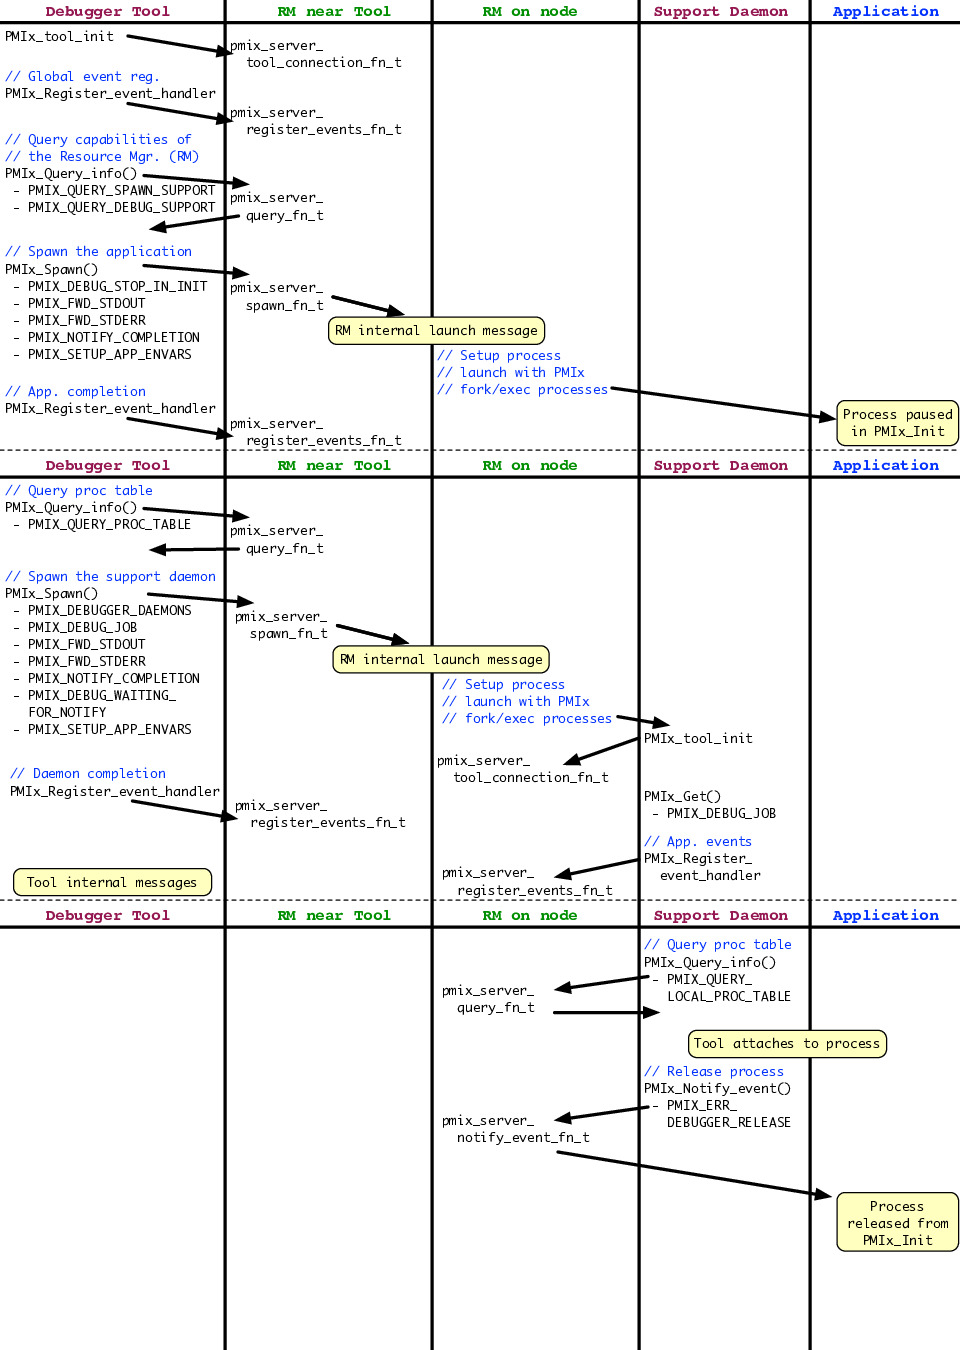
\includegraphics[width=\textwidth,height=\textheight,keepaspectratio]{figs/direct-launch}
  \end{center}
  \caption{Direct Launch}
  \label{fig:direct_launch}
\end{figure*}
\endgroup


\littleheader{Related Interfaces}

{\large \refapi{PMIx_tool_init}}
\pasteSignature{PMIx_tool_init}

{\large \refapi{PMIx_Register_event_handler}}
\pasteSignature{PMIx_Register_event_handler}

{\large \refapi{PMIx_Query_info}}
\pasteSignature{PMIx_Query_info}

{\large \refapi{PMIx_Spawn}}
\pasteSignature{PMIx_Spawn}

{\large \refapi{PMIx_Get}}
\pasteSignature{PMIx_Get}

{\large \refapi{PMIx_Notify_event}}
\pasteSignature{PMIx_Notify_event}

\littleheader{Related Attributes}

\pasteAttributeItem{PMIX_QUERY_SPAWN_SUPPORT}
\pasteAttributeItem{PMIX_QUERY_DEBUG_SUPPORT}
\pasteAttributeItem{PMIX_DEBUG_STOP_IN_INIT}
\pasteAttributeItem{PMIX_FWD_STDOUT}
\pasteAttributeItem{PMIX_FWD_STDERR}
\pasteAttributeItem{PMIX_NOTIFY_COMPLETION}
\pasteAttributeItem{PMIX_SETUP_APP_ENVARS}
\pasteAttributeItem{PMIX_DEBUGGER_DAEMONS}
\pasteAttributeItem{PMIX_DEBUG_JOB}
\pasteAttributeItem{PMIX_QUERY_LOCAL_PROC_TABLE}

\littleheader{Related Constants}

\refconst{PMIX_DEBUG_WAITING_FOR_NOTIFY} \\
\refconst{PMIX_DEBUGGER_RELEASE}

\subsubsection{Indirect-Launch Debugger Tool}

Executing a program under a tool using an intermediate launcher such as mpiexec can also be made possible. This requires some degree of coordination between the tool and the launcher. Ultimately, it is the launcher that is going to launch the application, and the tool must somehow inform it (and the application) that this is being done in a debug session so that the application knows to ``block'' until the tool attaches to it.

In this operational mode, the user invokes a tool (typically on a non-compute, or ``head'', node) that in turn uses mpiexec to launch their application – a typical command line might look like the following: \code{dbgr -dbgoption mpiexec -n 32 ./myapp}.

\begingroup
\begin{figure*}
  \begin{center}
    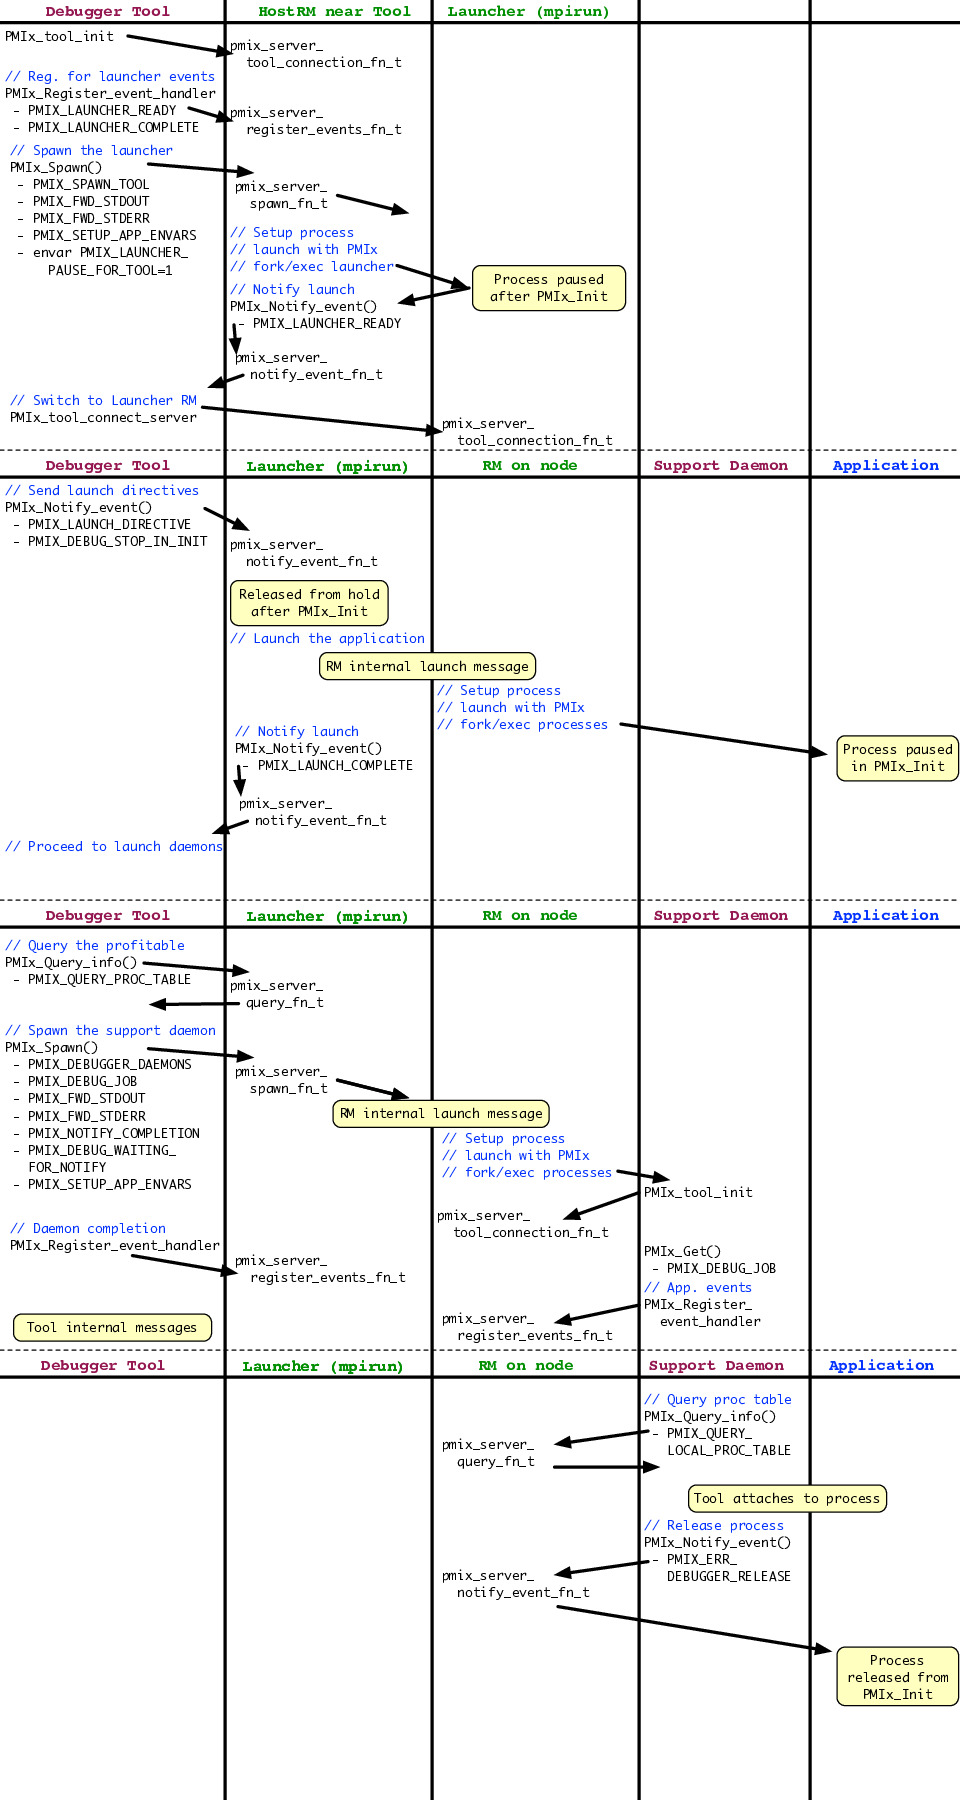
\includegraphics[width=\textwidth,height=\textheight,keepaspectratio]{figs/indirect-launch}
  \end{center}
  \caption{Indirect Launch}
  \label{fig:indirect_launch}
\end{figure*}
\endgroup


\littleheader{Related Interfaces}

{\large \refapi{PMIx_tool_init}}
\pasteSignature{PMIx_tool_init}

{\large \refapi{PMIx_Register_event_handler}}
\pasteSignature{PMIx_Register_event_handler}

{\large \refapi{PMIx_Spawn}}
\pasteSignature{PMIx_Spawn}

{\large \refapi{PMIx_Notify_event}}
\pasteSignature{PMIx_Notify_event}

{\large \refapi{PMIx_tool_attach_to_server}}
\pasteSignature{PMIx_tool_attach_to_server}

{\large \refapi{PMIx_Query_info}}
\pasteSignature{PMIx_Query_info}

{\large \refapi{PMIx_Get}}
\pasteSignature{PMIx_Get}

\littleheader{Related Attributes}

\pasteAttributeItem{PMIX_SPAWN_TOOL}
\pasteAttributeItem{PMIX_FWD_STDOUT}
\pasteAttributeItem{PMIX_FWD_STDERR}
\pasteAttributeItem{PMIX_SETUP_APP_ENVARS}
\pasteAttributeItem{PMIX_DEBUG_STOP_IN_INIT}
\pasteAttributeItem{PMIX_QUERY_PROC_TABLE}
\pasteAttributeItem{PMIX_DEBUGGER_DAEMONS}
\pasteAttributeItem{PMIX_DEBUG_JOB}
\pasteAttributeItem{PMIX_FWD_STDOUT}
\pasteAttributeItem{PMIX_FWD_STDERR}
\pasteAttributeItem{PMIX_NOTIFY_COMPLETION}
\pasteAttributeItem{PMIX_SETUP_APP_ENVARS}
\pasteAttributeItem{PMIX_DEBUG_JOB}
\pasteAttributeItem{PMIX_QUERY_LOCAL_PROC_TABLE}

\littleheader{Related Constants}

\refconst{PMIX_LAUNCHER_READY} \\
\refconst{PMIX_LAUNCH_DIRECTIVE} \\
\refconst{PMIX_LAUNCH_COMPLETE} \\
\refconst{PMIX_DEBUG_WAITING_FOR_NOTIFY} \\
\refconst{PMIX_DEBUGGER_RELEASE}

\subsubsection{Attaching to a Running Job}

PMIx supports attaching to an already running parallel job in two ways.  In the first way, the main process of a tool calls \refapi{PMIx_Query_info} with the \refattr{PMIX_QUERY_PROC_TABLE} attribute.  This returns an array of structs containing the information required for \hyperref[subsubsec:process-acq]{process acquisition}.  This includes remote hostnames, executable names, and process IDs.  In the second way, every tool daemon calls \refapi{PMIx_Query_info} with the \refattr{PMIX_QUERY_LOCAL_PROC_TABLE} attribute.  This returns a similar array of structs but only for processes on the same node.

An example of this use-case may look like the following: \code{mpiexec -n32~./myApp \&\& dbgr attach \$!}.

\begingroup
\begin{figure*}
  \begin{center}
    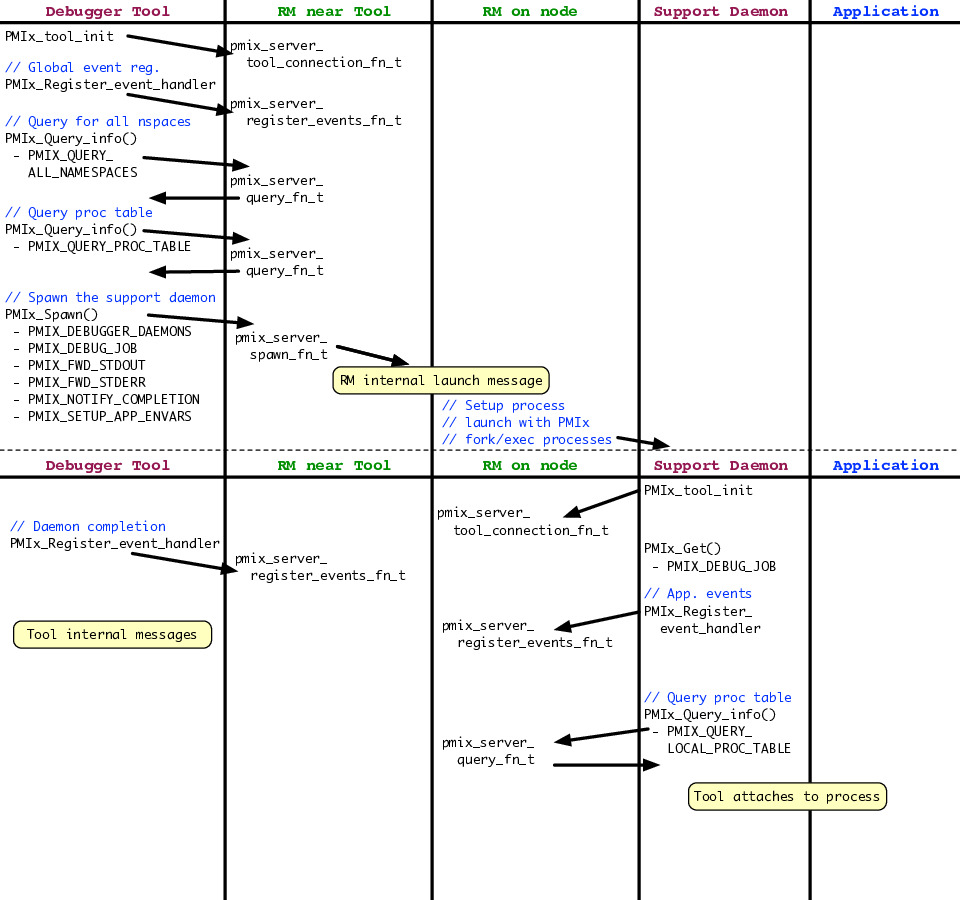
\includegraphics[width=\textwidth,height=\textheight,keepaspectratio]{figs/process-acquisition}
  \end{center}
  \caption{Attaching to a Running Job}
  \label{fig:proc_acq}
\end{figure*}
\endgroup

{\large \refapi{PMIx_tool_init}}
\pasteSignature{PMIx_tool_init}

{\large \refapi{PMIx_Register_event_handler}}
\pasteSignature{PMIx_Register_event_handler}

{\large \refapi{PMIx_Query_info}}
\pasteSignature{PMIx_Query_info}

{\large \refapi{PMIx_Spawn}}
\pasteSignature{PMIx_Spawn}

\pasteAttributeItem{PMIX_QUERY_PROC_TABLE}
\pasteAttributeItem{PMIX_DEBUGGER_DAEMONS}
\pasteAttributeItem{PMIX_DEBUG_JOB}
\pasteAttributeItem{PMIX_FWD_STDOUT}
\pasteAttributeItem{PMIX_FWD_STDERR}
\pasteAttributeItem{PMIX_NOTIFY_COMPLETION}
\pasteAttributeItem{PMIX_SETUP_APP_ENVARS}

\pasteAttributeItem{PMIX_QUERY_NAMESPACES}

\subsubsection{Tool Interaction with RM}

Tools can benefit from a mechanism by which they may interact with a local PMIx server that has opted to accept such connections along with support for tool connections to system-level PMIx servers, and a logging feature. To add support for tool connections to a specified system-level, PMIx server environments could choose to launch a set of PMIx servers to support a given allocation - these servers will (if so instructed) provide a tool rendezvous point that is tagged with their pid and typically placed in an allocation-specific temporary directory to allow for possible multi-tenancy scenarios. Supporting such operations requires that a system-level PMIx connection be provided which is not associated with a specific user or allocation. A new key has been added to direct the PMIx server to expose a rendezvous point specifically for this purpose.

{\large \refapi{PMIx_Query_info_nb}}
\pasteSignature{PMIx_Query_info_nb}

{\large \refapi{PMIx_Register_event_handler}}
\pasteSignature{PMIx_Register_event_handler}

{\large \refapi{PMIx_Deregister_event_handler}}
\pasteSignature{PMIx_Deregister_event_handler}

{\large \refapi{PMIx_Notify_event}}
\pasteSignature{PMIx_Notify_event}

{\large \refapi{PMIx_server_init}}
\pasteSignature{PMIx_server_init}

\littleheader{Job-specific events}
\code{PMIX_EVENT_JOB_LEVEL       /* debugger attached, process failure */}

\littleheader{Environment events}
\code{PMIX_EVENT_ENVIRO_LEVEL  /*ECC errors, temperature excursions */}

\littleheader{Errors detected by clients/peers}
\code{Network fabric manager detects data corruption}

\subsubsection{Environmental Parameter Directives for Applications and Launchers}

It is sometimes desirable or required that standard environmental variables (e.g., \code{PATH}, \code{LD_LIBRARY_PATH}, \code{LD_PRELOAD}) be modified prior to executing an application binary or a starter such as mpiexec - this is particularly true when tools/debuggers are used to start the application. This RFC proposes the definition of a new PMIx structure (\refstruct{pmix_envar_t}) and associated attributes for specifying such operations.

\littleheader{Related Interfaces}

{\large \refapi{PMIx_Spawn}}
\pasteSignature{PMIx_Spawn}

\littleheader{Related Structs}

\refstruct{pmix_envar_t}

\littleheader{Related Attributes}

\pasteAttributeItem{PMIX_SET_ENVAR}
\pasteAttributeItem{PMIX_ADD_ENVAR}
\pasteAttributeItem{PMIX_UNSET_ENVAR}
\pasteAttributeItem{PMIX_PREPEND_ENVAR}
\pasteAttributeItem{PMIX_APPEND_ENVAR}

Resource managers and launchers must scan for relevant directives, modifying environmental parameters as directed. Directives are to be processed in the order in which they were given, starting with job-level directives (applied to each app) followed by app-level directives.

%%%%%%%%%%%%%%%%%%%%%%%%%%%%%%%%%%%%%%%%%%%%%%%%%
